\section{Feature Extraction}
\par For the task of Dense Video Captioning, a rich feature space would enhance the representational power of the model, thereby leading to more meaningful and accurate event proposals and captions. In most previous works, convolutional neural networks are commonly used to extract features  from videos for any downstream tasks. Moreover, most localization methods use video features extracted by models that are trained for the task of Trimmed Action Classification (TAC), on datasets such as Kinetics\cite{kay2017kinetics} and Sports-1M, such as R(2+1)D\cite{r(2+1)d}, I3D\cite{carreira2018quo}, C3D and others. Additionally, most previous works focus on using a single modality (i.e. video) or multiple modalities based only on video, like RGB and optical flow features, for example from I3D\cite{carreira2018quo}, to generate feature vectors as input to the downstream model. Some works have used multiple modalities including video (RGB, optical flow) and audio, like \cite{iashin2020better}. The motivation for using multiple modalities is so that the feature space can grow richer, and that multiple modalities can complement each other to give strong event indicators. 

\par In this section, we explain how features are extracted from videos in the form of two modalities: video and audio. We use the \textit{Video Vision Transformer (ViViT)} \cite{vivit} for video feature extraction and the \textit{Audio Spectogram Transformer (AST)} \cite{ast} for audio feature extraction. We also consider the temporal sensitivity of features as a characteristic that can benefit DVC.

\subsection{Feature Extraction Methodology}


\subsubsection{Video Features Extraction Using ViViT} \label{video-feat-extraction}
\par Video features are the most important part of the encoder. Without a robust and rich feature space for videos, the downstream model would never be able to learn accurate event boundaries or captions. Previous state-of-the-art video encoders \cite{carreira2018quo}, \cite{csn}, \cite{r(2+1)d} use CNN-based architectures. Although they have strong inductive bias and translation invariance, they fail to model long-range temporal dependencies which are of importance when encoding videos. Moreover, CNNs require different architectures to model different modalities which can become complex when combining multiple modalities such as video and audio. Transformers \cite{tfm} can overcome these barriers using their attention mechanism without compromising on statistical and computational efficiency. Moreover, transformers can use the same building blocks across different modalities without many modifications. We aim to use the recently proposed ViViT model \cite{vivit}, a purely attention-based video encoder which has outperformed previous approaches for action recognition such as  Kinetics 400 and 600, Epic
Kitchens 100, Something-Something v2 and Moments in Time. Even though ViViT requires several orders of magnitude more training data as compared to its CNN counterparts, the authors of ViViT propose several methods to limit its training requirements by using pretrained weights in conjunction with strong regularization and specific fine-tuning.

\begin{figure} [H]
	\centering
	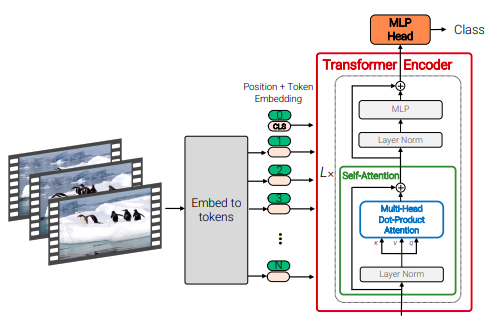
\includegraphics[width=7cm, height=6cm] {assets/img/vivit_methodology.png}
	\caption{ViViT encoder by Dosovitskiy \textit{et al}. (Image courtesy \cite{vivit})}
\end{figure}

% TODO: Working of VIVIT, video frames augmentation and preprocessing

\par Arnab \textit{et al} propose two methods for mapping a video to its corresponding embeddings for input to ViViT, \textit{Uniform frame sampling} and \textit{Tubelet embedding} in \cite{vivit}. We use the uniform frame sampling method in our feature extraction framework. Arnab \textit{et al} also propose different attention mechanisms for the ViViT model; we use the \textit{spatio-temporal attention} mechanism. The flow of data is as follows:

\begin{enumerate}
	\item Consider the original video clip $X$ as consisting of $T$ frames, each of width $W$ and height $H$. The video has $C$ channels. Hence the shape of video frames of $X$ is $(T, H, W, C)$.
	\item We perform certain preprocessing steps on the video frames:
	\begin{enumerate}
		\item We resize the spatial dimensions of the video frames. The shorter edge is resized to $256$, and the longer edge is resized maintaining the aspect ratio.
		\item We normalize all channels of the video frames.
		\item Generalizability and robustness of the features motivate data augmentation of the video frames. To this end, we randomly flip the video frames horizontally, and take random crops of spatial dimensions $224 \times 224 $ during training. Note that for validation and inference, we skip the random horizontal flip step and take a center crop of the same dimensions.
	\end{enumerate}
	\item Now, the uniform frame sampling method proposed by Arnab \textit{et al} in 
\cite{vivit} is used to extract tokens mapped to a $768$-dimensional space. This involves using a three-dimensional convolutional layer to project the frames to patch embeddings, so that the shape of the embeddings are $(T, N, 768)$, where $N$ is the number of patches.
	\item The patch embeddings are then flattened to $(T \times N, 768)$, and concatenated with a \textit{class token} for input to the encoder layers of ViViT.
	\item For each encoder layer, the input is first subject to positional encoding, followed by layer normalization, followed by multi-head self-attention across all tokens.
	\item Finally, the class token from the output of the last encoder layer is used as the feature representation of the clip $X$.
\end{enumerate}

\par More details about the different frame sampling methods, attention mechanisms and the ViViT model are given in \ref{appendix:vivit-paper}

\subsubsection{Audio Features Extraction using AST} \label{audio-feats-extraction}
\par Audio is an important aspect of any video. Not only does audio suggest the duration of an event, it can also signify the magnitude or significance of that event. Thus, audio becomes a powerful accessory to images when representing a video. We aim to use the recently proposed Audio Spectogram Transformer (AST) \cite{ast} which has outperformed current state-of-the-art models in audio classification.
\begin{figure} [H]
	\centering
	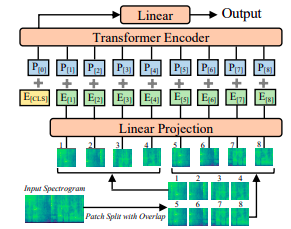
\includegraphics[width=7cm, height=6cm] {assets/img/ast_methodology.png}
	\caption{AST encoder by Gong \textit{et al}. (Image courtesy \cite{ast})}
\end{figure}

% TODO: Working of AST, Mel Spectograms and audio preprocessing

\subsection{Temporal Sensitivity of Features}
\par As mentioned previously, most localization methods use video features extracted by models that are trained for Trimmed Action Classification (TAC) tasks. These features are not necessarily optimal for Temporal Action Localization (TAL) and other dependent tasks such as Action Proposal Generation and Dense Video Captioning. Alwassel \textit{et al}, in their paper titled \textit{TSP: Temporally Sensitive Pretraining of Video Encoders for Localization Tasks}, claim that this is due to the inherent lack of temporal sensitivity in features from TAC trained video encoders \cite{alwassel2021tsp}. Yet, these features are prominently used for TAL and DVC tasks. This discrepancy is explained by the following reasons:
\begin{itemize}
	\item Due to a lot of existing research for TAC tasks, a lot of established models exist that can be used off the shelf for video feature extraction
	\item The video encoders usually cannot be directly trained along with downstream tasks of TAL or DVC due to resource constraints; it is impractical to fit long untrimmed videos in commodity GPUs without drastically downsampling them in terms of space or time.
\end{itemize}

\par To solve this problem, Alwassel \textit{et al} introduced a supervised pre-training paradigm for TAL that aims to instill the ability to produce temporally sensitive features; video encoders are trained to explicitly discriminate between foreground and background clips in untrimmed videos. They show that TSP improves performance for TAL, action proposal and DVC tasks consistently on different datasets as well as with different downstream predictive models and architectures, clearly establishing that temporally sensitive features contribute positively to the task at hand. TSP involves training encoders with a downstream task involving two classification heads: (1) \textit{action classification} head and (2) \textit{temporal region classification} head. This architecture is applied to clips from untrimmed videos. Optionally, along with local features of every clip, a \textit{global video feature (GVF)} is also used for the temporal region classification to further improve temporal sensitivity \cite{alwassel2021tsp}. A summary of their work is given in \ref{appendix:tsp-paper}.


\subsubsection{Temporally Sensitive Pretraining of Proposed Feature Extractors}

\par We extend the TSP framework proposed by Alwassel \textit{et al} \cite{alwassel2021tsp} to use temporally sensitive features in our work for DVC.

\paragraph{Architecture} The model used for TSP consists of one or more \textit{backbone} architectures for particular modalities, which in our case are ViViT - for video modality, and AST - for audio modality. The constructed model is such that different backbones and their modalities can be plugged in and out as required for experimentation. The input modality data of a clip is fed in to each backbone separately, and the output feature representations from each backbone are combined and passed through a fully connected layer to give a final feature representation. This feature representation is fed into the action classification head and the temporal region classification head to give the respective outputs. Note that we do not use a GVF in the current implementation of our pretraining framework, and plan to include this in later work.

\begin{figure}
\centering
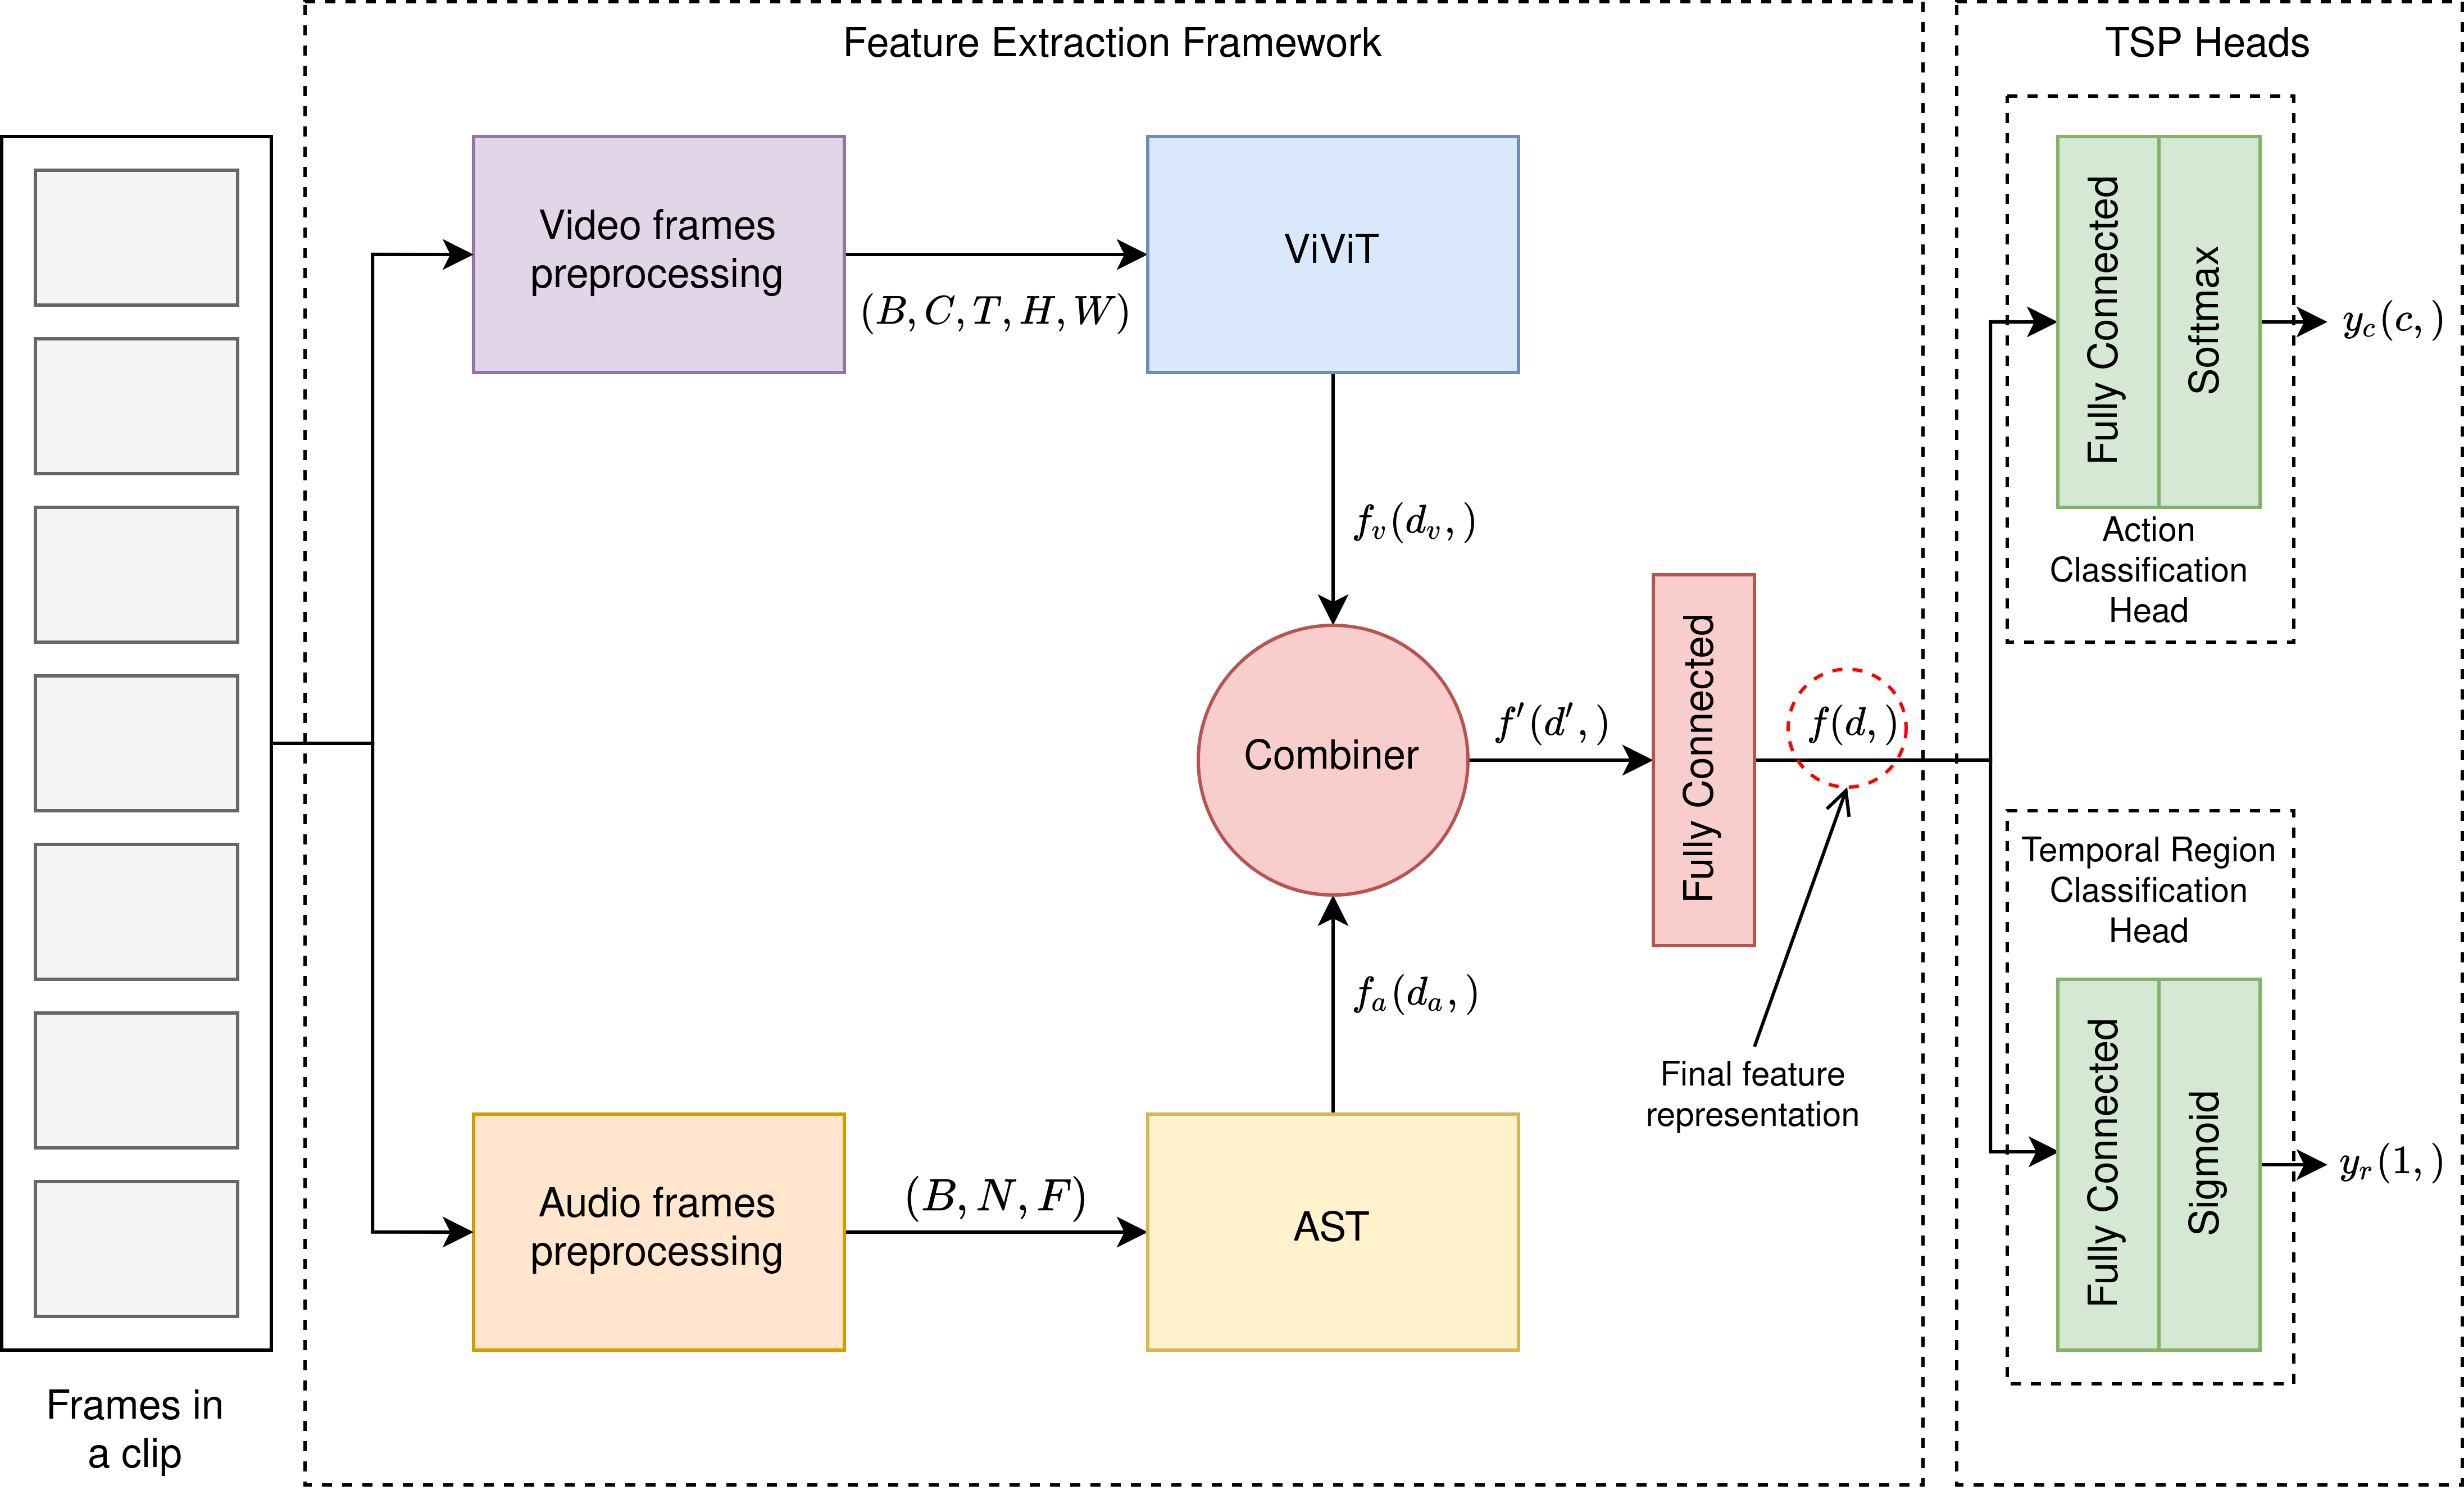
\includegraphics[width=\linewidth]{assets/img/tsp/tsp-arch.png}
\caption{The proposed feature extraction framework with ViViT and AST backbones. TSP heads for action classification and temporal region classification are shown on the right.}
\label{fig:tsp-arch}
\end{figure}

\paragraph{Data Flow} In our case, the following data flow is followed (considering two backbones: ViViT and AST):
\begin{enumerate}
	\item Video frames are extracted from the clips, and are preprocessed and augmented as mentioned in \ref{video-feat-extraction} making the features at this level of the shape $(B, C, T, H, W)$, where $B$ is the batch size, $C$ is the number of channels (3 for RGB), $T$ is the temporal length of the clip in terms of number of frames and $H$ and $W$ are the height and width (spacial dimensions) of each frame in the clip respectively.
	\item Audio frames are extracted from the clips as explained in \ref{audio-feats-extraction}. At this stage, they are of the shape $(B, N, F)$, where $N$ is the number of time frames and $F$ is the frequency bins.
%TODO Check AST dims and meanings
	\item Video features of the shape $(B, C, T, H, W)$ are fed into ViViT, and the class token of shape $(d_v, )$ of ViViT is used as the feature representation $f_v$ of the video modality of the clip.
	\item Audio features of the shape $(B, N, F)$ are fed into AST, and the class token of the shape $(d_a, )$ of AST is used as the feature representation $f_a$ of the audio modality of the clip.
	\item These two features, $f_a$ and $f_v$, are then combined using some function, for example addition or concatenation. In general, if there are $n$ backbones and we have features $f_1, f_2, f_3, ..., f_n$, this combiner function must combine all these and give a single-dimensional feature $f'$ of dimensions $(d', )$. 
	\item The feature $f'$ is fed into a fully connected layer that converts it into a feature $f$ of shape $(d, )$. This feature $f$ is the final feature representation that is used for downstream tasks.
	\item $f$ is fed to the action classification head, which consists of a simple fully connected layer followed by softmax activation layer, to give the action classification logits $y_c$ as output.
	\item $f$ is also fed (optionally combined with the GVF, $f_g$, to improve the temporal sensitivity of the feature representation) to the temporal region classification head, which consists of a fully connected layer followed by the sigmoid activation layer, to give the binary temporal region classification logit $y_r$ as output.
\end{enumerate}
\par The global video feature is extracted in the same manner as local features, with the additional step of \textit{pooling} across all local features ${f_1, f_2, ..., f_n}$ for a video. 

\paragraph{Loss functions} As mentioned, there are two classification heads on the top of the TSP framework:
\begin{itemize}
	\item \textbf{Action Classification}: This head predicts action classes for a given input clip. The head can be represented as $f \rightarrow y_c$. The cross-entropy loss function is used for this head, with mean reduction ($L_c$):
$$ L_{CE} = -\frac{1}{n} \sum_{i=1}^{n}{\textbf{y}log(\hat{\textbf{y}})} $$
	\item \textbf{Temporal Region Classification}: This head predicts temporal region classes for a given input clip, i.e. whether the particular clip lies in an action (foreground) temporal region or non-action (background) temporal region. The head can be represented as $f \rightarrow y_r$. For binary classification, the cross entropy function reduces to binary cross entropy ($L_r$).
\end{itemize}
\par The two losses, $L_c$ and $L_r$ are given loss coefficients $\alpha_c$ and $\alpha_r$ for relative importance for contributing towards the total loss:
$$ L = \alpha_c L_c + \alpha_r L_r $$

\par We evaluate the effectiveness of this temporally sensitive pretraining in the Results section.
%TODO Make results a ref, and add TSP eval

